% !Mode:: "Tex:UTF-8"
\chapter{结构感知的CNF混淆算法}
\label{chap:3}

\section{引言}%
软硬件设计验证过程中,通过Tseitin编码\upcite{Tseitin}将硬件电路、软件代码及待验证属性转化为统一的CNF
%(Conjunctive Normal Form)
公式,并进行SAT求解,以判断系统是否具有指定特性或是符合规定要求。
SAT求解问题是面向位级的,解空间随软硬件系统规模成指数级增长,对计算能力的扩展性要求高,适合部署在能够提供弹性计算资源的开放环境下。
但是,
研究表明,
虽然电路在Tseitin编码过程中损失了很多有用的逻辑信息,编码后生成的CNF公式中仍然携带了硬件电路结构等敏感信息;
另一方面,由于SAT问题的结果反映待验证属性是否符合预期,直接影响设计方案的成败,因此错误结果也是不可容忍的。

为避免开放环境下可能出现上述问题,本章以电路设计验证中SAT问题为研究对象,对系统进行建模,分析其中存在的安全威胁,并进而在此基础上提出了基于CNF 混淆的安全可验证SAT求解方法。在从理论上证明混淆算法的正确性之后,本文选取ISCAS89中的典型电路,对算法进行了性能测试和评估。

\section{问题描述}
本节将以云计算环境为例,
来建立开放环境下SAT求解的系统模型,并分析其中的安全威胁。
在研究中,存在两种类型的云,私有云和公共云:
\begin{enumerate}
\item 私有云是可信的,表现在两方面,一是数据的隐私性可以得到保证,二是计算结果的正确性可以确认;但私有云的计算及存储能力受限,仅仅适合处理对计算资源需求量小且相对稳定的简单计算。
\item 公共云可以提供弹性的计算及存储资源,适合承担计算资源需求量大的复杂计算任务;
但由于公共云处于互联网环境下,这种开放计算环境存在中存在诸多安全威胁,
如“诚实但好奇”的计算参与者,
这些计算参与者会尽力完成所有的计算任务,获得正确的结果,但是它们会试图获取计算数据中隐藏的信息。
\end{enumerate}

传统的综合与验证工具的核心框架通常包含以下主要功能模块:
\begin{enumerate}
\item 抽象问题表示:该模块用于管理与特定推理过程和引擎无关,但是与问题本身密切相关的数据结构,如Reduced Boolean circuits\upcite{DBLP:conf/tacas/AbdullaBE00}和And-Inverter Graph\upcite{Brummayer06localtwo-level} 等。
\item 问题编码:该模块用于将特定的抽象问题表示,转换为满足特定推理引擎,如二叉决策图(BDD) 或可满足问题(SAT)要求的数据结构,以便进行高效的推理工作。
针对SAT,该模块通常使用在空间和时间方面均具有多项式复杂性的Tseitin\upcite{Tseitin}编码。
\item 二叉决策图(BDD)和SAT推理引擎:这两个模块负责具体的推理工作。
\end{enumerate}

基于对形式化验证\upcite{DBLP:conf/atva/ShenQL04,DBLP:conf/vmcai/ShenQL05,DBLP:conf/date/ShenQL05,
DBLP:conf/charme/ShenQL05,DBLP:conf/aspdac/ShenQL05}和对偶电路综合\upcite{DBLP:conf/iccad/ShenZQL09,
DBLP:journals/tcad/ShenQWXZL10,DBLP:conf/iccad/ShenQZ11,DBLP:journals/tcad/ShenQWXZL10,
DBLP:journals/tcad/ShenQXWZL11,DBLP:journals/tcad/ShenQWPZL12}方面的研究,
发现一个通常的综合验证问题可以简述为:将硬件网表和需要验证的属性通过抽象问题表示和问题编码转换为BDD或CNF 公式,然后使用BDD推理引擎或SAT推理引擎对公式进行推理并返回结果。

抽象问题表示和问题编码转换通常是多项式复杂度的,计算开销相对稳定;
BDD受到归一化表示方式导致的状态空间爆炸问题的困扰,通常仅用于需要归一化特性的小规模推理问题,如抽象迁移关系的构造和精炼\upcite{softwareSAT}等;因此这两类计算适合部署在私有云环境下。
SAT则通常较少受到状态空间爆炸的影响,且天生具有内在的并行性和可扩展性,因此较为适合运行于公有云的核心推理引擎。

结合这些情况,CNF公式将在私有云中产生,SAT求解器部署在公共云,用于求解CNF公式,并将结果返回给私有云。
由于公共云环境下存在“诚实但好奇”的计算参与者,
他们会尽力完成所有的计算任务以便获得正确的CNF公式的解,
但是它们也试图从CNF公式或解中获得他们需要的信息,例如电路结构信息。
文献\upcite{csLiequivalency,csOstrowski,csRoy,csFu}
研究了抽取和利用CNF公式中电路结构信息的方法。
Roy等人\upcite{csRoy}和Fu等人\upcite{csFu}给出了基于子图同构以及模式匹配的电路结构抽取算法,
并能最大限度的恢复出CNF公式中的电路结构。这些技术可能会被潜在的攻击者利用来抽取敏感的电路结构信息。
因此,CNF公式包含的结构信息应该被当做隐私加以保护。

\section{基于CNF混淆的SAT求解方法}

\subsection{SAT求解框架}
设计基于开放环境下SAT求解框架,将考虑下面三个因素:

\begin{enumerate}
 \item 可移植性:目前的SAT求解器集成了冲突检测\upcite{EFFCON}等高效机制,
 因此我们希望可以将其作为黑盒直接使用,
 而不是像\upcite{OBfuscationd-CNFs} 等基于全同态的方案那样,需要重新构造问题并试图使用新的求解算法。
 \item \label{3:g2} 隐形性\upcite{obfuscationBible}:求解框架应该保护CNF公式中的电路结构不会被获取。
\item 结果可验证:计算结果可以验证。
 \item \label{3:g3} 开销:框架不应该引入太多的开销。
\end{enumerate}

上面的要求具体说来可以归结为这样一个有趣的问题:
将SAT 问题编码为CNF公式外包到云中,由未经修改的经典SAT求解器求解;
并且不希望SAT求解器知道实际SAT问题的原始结构。

直觉来看,
一个简单的方法就是将原始CNF公式$F_C$和一个与其无变量交集的可满足公式$F_H$,
简单混合在一起,
并将混合后的CNF公式$F_C\wedge F_H$外包的云上。
由于可满足公式$F_H$必然存在解,
那么如果原始公式$F_C$有解,
其解将会混杂在混合后的解中。
这种方法非常简单易行.
但是,基于分区\upcite{Partition}的方法可以将两个不相关的公式分离开来,
从而得到原始CNF 公式$F_C$。

再来考虑一个改进的方法:
任意公式$F_C$和一个可满足公式$F_H$,
$F_C$和$F_H$没有公共变量, 也即:$V_{F_C}$ $\cap$ $V_{F_H}$ =$\phi$。
将$F_C$和$F_H$无缝混合以便于隐藏$F_C$;同时,保持$F_C$中的所有解都包含在新的公式中。
而要实现$F_C$和$F_H$无缝混合,需要实现两个公式子句的交织,
需要存在既包含$F_H$变量,同时又包含$F_C$变量的子句。
根据CNF公式的定义可知其具有如下特性:
对任意CNF公式$F_C$,在其子句中加入新的文字可能会扩展解空间;
而另一方面,
在$F_C$中加入包含$F_C$中变量的子句则会缩减解空间。

那么,
如何在此情况下保证$F_C$所有的解仍旧保留在新的公式中?
为了实现该目标,
本章给出了安全可验证的SAT求解框架。
为了混淆CNF公式$F_C$,
根据后续章节介绍的SSH规则策略,
采用随机的方式在公式$F_C$的子句中加入新的文字,
并根据加入的文字在公式中加入新的子句。
新加入的文字和一部分新的子句来自于被称为单一Husk公式$F_H$(见定义\ref{3:Singular-Husk-formula-definition})的噪音公式。
SSH规则保证原始CNF公式$F_C$可以和单一Husk公式$F_H$无缝地混合在一起,
达到\ref{3:g2}) 和 \ref{3:g3})的要求。
%SSH规则和CSA策略将在\textit{\ref{3:embeded rules})} 和 \textit{\ref{3:embeded strategy})} 小节中介绍。

\begin{definition}[单一Husk 公式]\label{3:Singular-Husk-formula-definition}
单一Husk公式是仅有一个可满足解的CNF公式,
并且解中变量的赋值是非特异的,即他们不是全$T$或全$F$。
\end{definition}

框架的详细实现在图 \ref{3:fig_cldSAT}中给出。
在该框架下, SAT问题的求解包含了以下4步。
\begin{itemize}
\item \textbf{步骤 1}:产生器产生一个单一Husk公式$F_H$和它的一个解$R_H$。
\item \textbf{步骤 2}:混淆器将原始CNF公式$F_C$和单一Husk公式$F_H$混合,并产生一个新的CNF 公式$F_O:=F_H\wedge F_C$。
\item \textbf{步骤 3}:$F_O$由位于公共云上的SAT求解器求解,并返回结果$S_O$。
\item \textbf{步骤 4}:映射器从$S_O$中抽取出$S_C$,验证器确认$S_C$是$F_C$的解。
\end{itemize}


\begin{figure}
\footnotesize\centering
\centerline{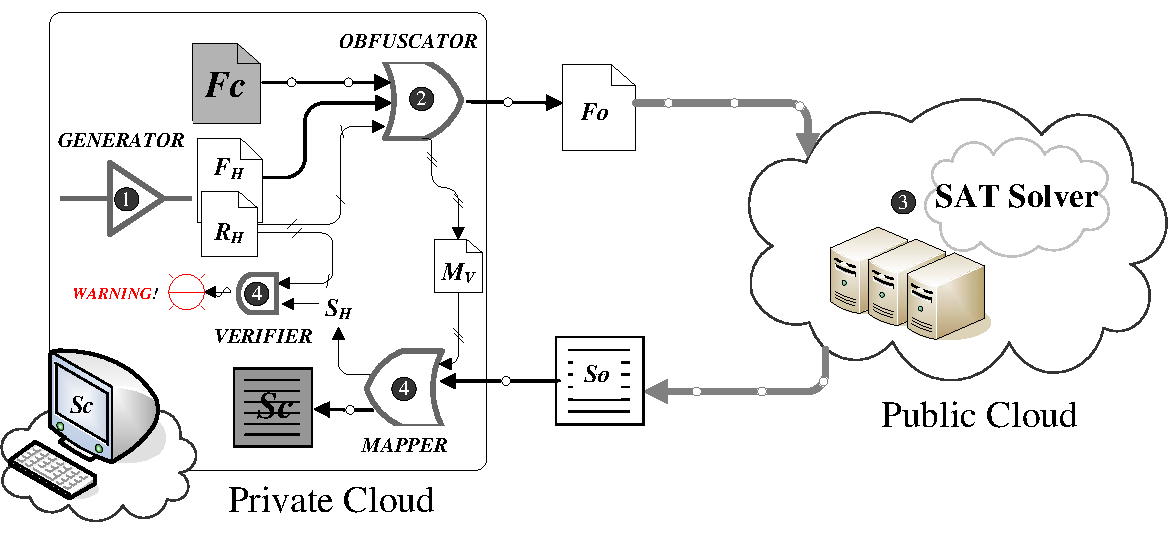
\includegraphics[width=12.2cm]{fig301}}
\caption{基于CNF公式混淆的安全可验证SAT求解框架}
%\caption{Privacy-preserving SAT solving framework based on CNF formula obfuscation.}
\label{3:fig_cldSAT}
\end{figure}

\textbf{步骤3}在开放环境下的公共云中运行,其余的步骤在可信的私有云上运行。
%
产生器,混淆器,映射器和验证器算法将在\ref{3:genhusk}, \ref{3:obfuscating}和\ref{3:mappping} 小节中分别介绍。




\subsection{单一Husk公式产生算法}\label{3:genhusk}

产生可满足CNF公式的算法有多种\upcite{microgenSAT,genSAT}.
仅有一个可满足解的单一Husk 公式(见定义\ref{3:Singular-Husk-formula-definition}) 采用质因数的方法构造\upcite{genSAT},
其中的具体实现在算法\ref{3:algo2_genSAT}中描述。

\textbf{首先},
给定质数$p_A$(第 \ref{3:primenumber}行),
% represented by a binary vector $p_A = <a_1,a_2,\dots,a_n>$, $p_B = <b_1,b_2,\dots,b_n>$,
将$p_A * p_A$ 赋值给乘法器$M$的输出,并且限制$I_1\ne 1$ and  $I_2\ne 1$ (第\ref{3:multiplePrime}行)。
其中,$I_1$和$I_2$ 是$M$的输入。

\textbf{第二},
将乘法器$M$编码为CNF公式$Tseitin(M)$(第\ref{3:TseitinPHI}行)。

为了满足$Tseitin(M)$,
$M$的两个输入的唯一解一定是$R_H:=\{I_1\equiv p_A,I_2\equiv p_A\}$。


%
 \begin{algorithm}[t]
 \caption{GENERATOR}
 \label{3:algo2_genSAT}
 \begin{algorithmic}[1]
 \STATE input : NULL;
 \STATE output : Husks CNF $F_H$ and Husks result $R_H$;
 \STATE Generating prime numbers $p_A$; \label{3:primenumber}
 \STATE $\Phi= M(I_1 \neq 1, I_2\neq 1, O=p_A*p_A)$ ;\label{3:multiplePrime}
 \STATE $F_H=Tseitin(\Phi)$ ;\label{3:TseitinPHI}
 \STATE $R_H=\{I_1\equiv p_A,I_2\equiv p_A\}$ ;
 \end{algorithmic}
 \end{algorithm}

\subsection{解空间保持的混淆算法}\label{3:obfuscating}
让我们继续考虑开篇提到的有趣问题:
如何将SAT问题编码为CNF 公式外包到云中,
由云端的SAT求解器求解;
并且不希望SAT求解器获知原始SAT问题的结构。
对来源于硬件验证的SAT问题而言,这个问题就具化为:
一方面,希望求解器无法获取原CNF公式携带的电路结构信息,可使用“抗结构感知”来描述这一特性;
而另一方面,希望求解器还能够给出正确解。这不仅包括解的取值是正确的,还包括解的个数也是正确的。
本文的后续使用“保持解空间”来描述这一特性。

\subsubsection{解空间保持规则}
%To prevent information carried by CNF formula and its solution from leakage, a privacy-preserving scheme is proposed,
%the scheme is based on the following facts and anticipations:
%\\$\textbf{Fact 1:}$ Changing CNF signature and key clause in CNF formula will make circuit recovering
%based on pattern matching or subgraph isomorphism impossible.
%\\$\textbf{Fact 2:}$ Solution space should not be under-approximated after obfuscation, otherwise the result will be misleading even for real user.
%\\$\textbf{Anticipation 1:}$ According to Fact 2, solution space have to be over-approximated  after obfuscation, so as to mislead hoarding participants in public Cloud.
%\\$\textbf{Anticipation 2:}$ The solution of obfuscated CNF formula should be easily mapped back to the original formula.
%为了防止CNF公式以及解的信息泄露,给出了一个隐私保护的策略,该策略基于下面的事实和期望:
%\\$\textbf{事实 1:}$ 改变公式中的CNF标记和关键子句可以使基于模式匹配或子图同构的电路结构恢复技术失效。
%\\$\textbf{事实 2:}$ 混淆后的解空间不应该被缩小,否则会误导真实应用,例如验证等。
%%\\$\textbf{期望 1:}$ 鉴于事实2, 解空间应该被扩大,以便于误导公共云上包括SAT求解器在内的第三方。
%\\$\textbf{期望 1:}$ 可以从混淆后的解中较快的恢复出原公式的解。

%本章在\textit{\ref{3:embeded rules}})介绍SSH规则。
%\subsubsection{解空间保持(SSH)规则}\label{3:embeded rules}

一个能同时实现“抗结构感知”和“解空间保持”的方法,
是将真实CNF公式$F_C$和一个在变量上和其无交集的可满足公式$F_H$,混合在一起,将混合后的CNF公式$F_O$外包的云上。
由于SAT求解器拿到的不是真实CNF公式,原始公式中包含的结构信息自然无从获得,这就实现了“抗结构感知”。
由于可满足公式$F_H$必然存在解,那么如果真实公式$F_C$有解,其解将会混杂在混合后公式$F_O$ 的解中,
混合后公式就是可满足的(SAT)。
而如果如果原始公式$F_C$没有解,混合后公式$F_O$也将是不可满足的(UNSAT)。
因此这种混合也是解空间保持的。
唯一不足的是,简单混合无法防止基于分区方法\upcite{Partition}的攻击。

改进的方法是
%任意公式$F_C$,和一个可满足公式$F_H$及其唯一解\textsl{${\textbf{R}}_{\textbf{H}}$},
%$F_C$和$F_H$没有公共变量, 也即:$V_{F_C}$ $\cap$ $V_{F_H}$ =$\phi$。
将原始CNF公式$F_C$和可满足公式$F_H$无缝混合,以便于隐藏$F_C$。
为实现$F_C$和$F_H$无缝混合,
直觉的方法是将$F_H$中的变量加入到$F_C$的子句中,
或使用$F_C$和$F_H$中的变量产生新的子句,这样就可以构造同时包含$F_C$和$F_H$中文字的子句。
但是根据CNF公式的定义可知其具有如下特性:
对任意CNF公式$F_C$,在子句中加入新的文字可能会扩展解空间;
而另一方面,
在$F_C$中加入包含$F_C$中变量的子句则会缩减解空间。
那如何在此情况下保证$F_C$的解仍旧保留在新的公式中?
在给出具体答案之前,首先澄清下面的概念。

\begin{definition}[解包含关系 $S_C \subseteq S_O$]
CNF 公式式$F_C$和$F_O$具有$n_{F_C}$个公共变量$x_1,...,x_{n_{F_C}}$ 。
并且有
$|V_{F_C}|\equiv n_{F_C}$, $|V_{F_O}|\equiv n_{F_O}$, $ n_{F_O}\geqslant n_{F_C} > 0$。
$S_C$和$S_O$分别是$F_C$和$F_O$的解。
在$S_C$和$S_O$中,$n_{F_C}$ 个公共变量的赋值是相同的, 也就是
$S_C=\{x_1=B_1,...,x_{n_{F_C}}=B_{n_{F_C}} | B_i \in \{T,F\},~1\leqslant i\leqslant n_{F_C} \}$,
$S_O=\{x_1=B_1,...,x_{n_{F_C}}=B_{n_{F_C}},...,x_{n_{F_O}}=B_{n_{F_O}}|B_i\in \{T,F\},~ 1\leqslant i\leqslant n_{F_O} \}$。
称解$S_C$包含于$S_O$,记为$S_C\subseteq S_O$。
\end{definition}

\begin{definition}[解空间等价(SSE)]\label{3:SSEdefinition}~
CNF公式$F_C$有$n$个解$\{S_{C_1},...,S_{C_n}\}$;
CNF公式$F_O$也有$n$个解$\{S_{O_1},...,S_{O_n}\}$,
并且对于任意$i \in [1,n]$, $S_{C_i} \subseteq S_{O_i}$。
称$F_O$解空间等价于$F_C$,记为$F_C \equiv_{_{SSE}} F_O$。
\end{definition}

为了在新公式中保持$F_C$公式中的所有解,
我们将在下面给出解空间保持(SSH)规则。
本章介绍的混淆器将使用SSH规则,
将Husks公式$F_H$嵌入到原始公式$F_C$中,产生一个新的CNF公式$F_O$。
这将防止攻击者通过模式识别或是子图同构技术获取公式中携带的电路结构信息。
SSH规则同时还将保证混淆后的解空间与原公式解空间等价。

\textbf{解空间保持(SSH)规则: }
\begin{enumerate}
\item[] \textbf{规则 1:子句替换规则}:
对任一子句$c\in F_{C}$,
从$R_H$中任取出变量$v$,
并按照下列规则插入到子句$c$中:
如果在$R_H$中变量$v$的赋值是$T$,则插入负文字$\neg v$;
如果在$R_H$中变量$v$的赋值是$F$,则插入正文字$v$;
用新生成的子句代替原始子句$c$。
\item[] \textbf{规则 2:子句生成规则}:
任取$R_H$中的文字和$F_C$ 中的变量创建新的子句。
\end{enumerate}

\begin{definition}[${\textbf{Obf(}}F_C,F_H,R_H\textbf{)}$]\label{3:OBFUSCATORSSH_old}
对任意公式$F_C$,和可满足公式$F_H$及其一个赋值$R_H$,
$Obf(F_C,F_H,R_H)$ 是在基于SSH规则将$F_C$和$F_H$混合后得到的公式。
\end{definition}

\begin{definition}[SSE混淆]\label{3:OBFUSCATORSSH}
如果$F_H$是单一Husk公式并且$R_H$是它的唯一解,
就称$Obf(F_C,F_H,R_H)$为解空间等价的混淆,称为${\textbf{SSE混淆}}$。

%如果$F_H$是Husks公式并且$R_H$是它其中一个解, 就称$Obf(F_C,F_H,R_H)$为${\textbf{SSO obfuscation}}$。
\end{definition}
% \begin{definition}[${\textbf{Obf(}}F_C,F_H,R_H\textbf{)}$]\label{3:OBFUSCATORSSH}
% For arbitrary formula $F_C$, and satisfiable formula $F_H$ with $R_H$ as one of its solutions,
% $Obf(F_C,F_H,R_H)$ is the result of applying SSH Rules when blending $F_C$ with $F_H$.
% If $F_H$ is a Singular Husk formula, $Obf(F_C,F_H,R_H)$ is called ${\textbf{SSE obfuscation}}$.
% If $F_H$ is Husks formula, $Obf(F_C,F_H,R_H)$ is called ${\textbf{SSO obfuscation}}$.
% \end{definition}

%For SSH based obfuscation, we have following theorems.
对基于SSH规则的${\textbf{SSE混淆}}$,下列定理成立。


\begin{theorem}[SSE Obfuscation]\label{3:SSEtheorem}
对任意CNF公式 $F_C$和单一Husk公式$F_{_SH}$,如果
~~$V_{F_C}$ $\cap$ $V_{F_{_SH}}$ =$\phi$, 并且
$R_{_SH}$是$F_{_SH}$的唯一解,
则 $Obf(F_C,F_{_SH},R_{_SH}) \equiv F_C\wedge F_{_SH}$。
\end{theorem}

基于定理\ref{3:SSEtheorem} 和定义\ref{3:SSEdefinition},有:

\begin{theorem}\label{3:SSEinference}
对任意CNF公式 $F_C$和单一Husk公式$F_{_SH}$,
如果有$V_{F_C}\cap V_{F_{_SH}}\equiv \phi$,
而且$R_{_SH}$是$F_{_SH}$的唯一解,
则 $Obf(F_C,F_{_SH},R_{_SH}) \equiv_{_{SSE}} F_C$。
\end{theorem}




定理\ref{3:SSEtheorem}和\ref{3:SSEinference}的严格证明将在\ref{3:correctness}小节给出。

%Theorem \ref{3:SSEtheorem} and \ref{3:SSOtheorem} will be proved in Subsection \ref{3:correctness}.
%An obfuscated CNF formula $F_O=Obf(F_C,F_H,R_H)$ generated by SSO obfuscation
%consists of all the variables of $F_C$ and $F_H$.

经过SSE混淆生成的CNF公式$F_O=Obf(F_C,F_{_SH},R_H)$,
包含了$F_C$和$F_{_SH}$中的所有变量;
并且根据SSH\textbf{规则1},
$F_C$中的部分子句被加入了$F_{_SH}$中的变量对应的文字,而成为了新的子句。
由于$F_{_SH}$解的非特异性,这些文字不全为正也不全为负;
还有部分子句是根据SSH\textbf{规则2},由分别取自$F_C$和$F_{_SH}$的变量文字组合而成。
从形式上看,$F_O$是一个合法的CNF公式。
而根据定理\ref{3:SSEtheorem},可知混合后公式$F_O$的解是$F_C$和$F_{_SH}$的交集。
由于公式$F_C$和$F_{_SH}$无公共变量,又由于$F_{_SH}$只有唯一解,
这就使得$F_O$的解的个数和$F_C$的一致。可以得到如下的结论:

%$F_H$中的变量被赋值为$R_H$,则有:
%
%$F_O(R_H/V_{F_O})
%=Obf(F_C,F_H(R_H/V_{F_H}),R_H)$
%
%根据引理\ref{3:SHE}(\ref{3:correctness}小节),
%$F_H(R_H/V_{F_H})$可以被表示为一个单一Husk公式,有唯一解$R_H$。
%根据推论\ref{3:SSEinference},对任意$F_C$和混淆后公式$F_O$,则有:
\begin{enumerate}
 \item $F_C$是不可满足的当且仅当$F_O$不可满足,
 并且 $F_C$的不可满足核可以通过从$F_O$的不可满足核中删除$F_H$中的文字获得。
 \item $F_C$可满足当且仅当$F_O$是可满足的,
 并且$F_C$的解可以通过将$F_O$的解投影到$F_C$的变量集中获得。
\end{enumerate}



综上所述,经过SSH混淆变换后,
$F_O$和$F_C$在形式上相似,
$F_O$和$F_C$可以使用同样的SAT求解器求解。
在不知晓$R_H$的情况下,$F_C$将很难被从$F_O$剥离;
另一方面,$F_O$的解空间和$F_C$解空间等价。
通过SSH规则,算法\ref{3:algo_obs}所示的混淆器OBFUSCATOR可以在子句中添加新文字并且创建新的子句,
同时保证解空间不被扩展或缩减;
这就实现了与全同态加密相似的混淆效果。


\subsubsection{\textsl{OBFUSCATOR 算法}}

OBUFSCATOR算法遵循上述SSH规则,混淆CNF公式$F_C$,从而防止$F_C$所携带的电路结构信息被潜在的攻击者获取。
SSH规则保证了解空间的不变。
如何达到隐藏电路结构信息的目的,则需要确定如何在子句中添加新的文字以及构造新的子句。

为了达到上述目标,OBFUSCATOR首先会在第$\ref{3:mark}$行使用算法\ref{3:algo_mark}中的mark算法,
得到CNF公式中的关键子句和输出文字集合,
以确定究竟选取哪些子句加入文字;
而后通过在关键子句中加入噪音文字,破坏原有的结构。
OBFUSCATOR的详细实现在算法\ref{3:algo_obs}中,


\begin{algorithm}[t]
\caption{$\mathbf{mark}$}
\label{3:algo_mark}
\begin{algorithmic}[1]
%\SetAlgoNoLine
\STATE $\mathbf{mark}$;
\STATE input : CNF formula $S$;
\STATE output : marked $S$ ;
\STATE $KeyClauseSet := \{\}$
\STATE $OutLiteralMap := \{\}$
\FOR{$(C \in S)$}
\IF{$|C|\equiv 2$}
\STATE $KeyClauseSet := KeyClauseSet\cup C$
\FOR{$(l \in C)$}
\STATE $OutLiteralMap := OutLiteralMap\cup (C,l)$
\ENDFOR
\ENDIF
\ENDFOR
\RETURN $(KeyClauseSet,OutLiteralMap)$
\end{algorithmic}
\end{algorithm}

\begin{algorithm}[t]
\caption{$\mathbf{generate\_new\_clause}$}
\begin{algorithmic}[1]
\STATE $\mathbf{generate\_new\_clause}$;
\STATE input : key clause $C$, Husk literal $lit$, $OutLiteralMap$;
\STATE output : new clause $C_1$;
\STATE 假设$(C,l)\in OutLiteralMap$
\STATE $C_1= lit \cup \neg l$ ;\label{3:rule2}
\end{algorithmic}
\end{algorithm}


\begin{algorithm}[t]
\caption{OBFUSCATOR}
\label{3:algo_obs}
%\SetAlgoNoLine
\begin{algorithmic}[1]
\STATE input : The original CNF $F_C$, Husks CNF $F_H$, Husks result $R_H$
\STATE output : The obfuscated CNF $F_O$, variable mapping $M$
\STATE $(KeyClauseSet,OutLiteralMap):=mark(F_C)$;\label{3:mark}
\FOR{$c\in F_C$}
\IF{$c \in  KeyClauseSet$} \label{3:keyclause}
\STATE     lit =get literal $ \in R_H$;
\STATE     $c=c \cup \neg lit$;\label{3:rule1}
\STATE     $nc=generate\_new\_clause(c,lit,OutLiteralMap)$;\label{3:gennewclause}
 \STATE    $F_C=F_C \cup nc$;\label{3:blendclause1}
\ENDIF
\ENDFOR
\FOR{$ c \in F_C $}
\STATE $averagelen=\frac{\sigma _{c'\in F_C}|c'|}{|F_C|}$ ;
\WHILE{$|c| < averagelen$}
\STATE $lit=$get literal $\in R_H$ ;
\WHILE{$\neg lit \in c$}
\STATE lit=get literal $ \in R_H $ ;
\ENDWHILE
\STATE $c=c \cup \neg lit$;\label{3:rule1-2}
\ENDWHILE
\STATE $M$ =remap all variable in $F_C\cup F_H$ ;\label{3:MV}
\STATE $F_O$ =reorder all clause in $F_C\cup F_H$ ; \label{3:blendclause2}
\ENDFOR
\end{algorithmic}
\end{algorithm}



%\begin{algorithm}[t]
%\caption{$\mathbf{mark}$ and $\mathbf{generate\_new\_clause}$}
%\label{3:algo_mark}
%\begin{algorithmic}[1]
%%\SetAlgoNoLine
%\STATE $\mathbf{mark}$;
%\STATE input : CNF formula $S$;
%\STATE output : marked $S$ ;
%\FOR{$(C \in S) ~\&~ (|C|\equiv 3)$}
%\FOR{$l \in C$ }
%\FOR{$(C_1 \in S) ~\&~ (\neg l\in C_1)~ \&~ (|C_1|\equiv 2)$ }
%\FOR{$l_1 \in C_1$ }
%\IF{$(\neg l_1 \in C)~\&~(l_1\ne l)$}
%\STATE $match++$ ;
%\ENDIF
%\ENDFOR
%\ENDFOR
%\ENDFOR
%\ENDFOR
%\IF{$match\equiv 2$}
%\STATE mark $l$ as output literal ;
%\STATE mark $C$ as Key Clause;
%\ENDIF
%


%\begin{algorithm*}[b]
%\caption{GENERATOR}
%\label{3:algo2_gen}
%\begin{algorithmic}[1]
%%%\SetAlgoLined
%%\SetAlgoNoLine
%\STATE input : NULL
%\STATE output : Husks CNF $F_H$ and Husks result $R_H$
%\STATE Generating prime numbers $p_A$ and $p_B$  ; \label{3:primenumber}
%\STATE $\Phi= M(I_1 \neq 1, I_2\neq 1, O=p_A*p_B)$ ;\label{3:multiplePrime3MVMV}
%\STATE $F_H=Tseitin(\Phi)$ ;\label{3:TseitinPHI}
%\STATE $R_H=p_A\mid p_B$ ;
%\end{algorithmic}
%\end{algorithm*}

\subsection{映射和验证算法}\label{3:mappping}
在公共云上的求解器完成求解后,将$F_O$的解$S_O$返回给私有云。
和混淆器相对应,在私有云中使用$MAPPER\_VERIFIER$将$F_C$ 的解从$S_O$中过滤出来。
$MAPPER\_VERIFIER$的实现在算法\ref{3:algo_map}中。

根据定理\ref{3:SSEtheorem},
如果结果是UNSAT, 那么原始的CNF公式也是(第\ref{3:sUNSAT}行)。
如果结果是SAT, 第\ref{3:var}-\ref{3:mapper} 行将解投影到$F_C$和$F_H$的变量上,
以获得$S_C$ 和$S_H$,分别作为$F_C$和$F_H$的候选解。
第\ref{3:verifer1}-\ref{3:verifer2} 行检测$S_H$是否等于$R_H$。
如果等于, $S_C$就是$F_C$的真实解。
否则,$S_C$是错误解,说明云端给出的结果是不可信的。

解的投影过程依赖于变量映射表$M$,它由OBFUSCATOR(算法\ref{3:algo_obs}的\ref{3:MV} 行)创建。
$M[var].variable$ (第\ref{3:var}行)表示了var 的原始变量名,
$M[var].formula$ (第\ref{3:formula}行)表示var所属于的公式,可以是$F_C$ 或 $F_H$。

\begin{algorithm}[t]
\caption{MAPPER-VERIFIER}
\label{3:algo_map}
%\SetAlgoNoLine
\begin{algorithmic}[1]
% \SetAlgoNoLine
\STATE input : Obfuscated result $S_O$, variable mapping table $M$, Husk result $R_H$;
\STATE output : Result $S_C$;
\IF{$S_O$ is UNSAT} \label{3:sUNSAT}
\RETURN UNSAT ;
\ENDIF
\FOR {$lit \in S_O$}
\STATE $var=abs(lit)$;
\STATE $rvar=M[var].variable $;\label{3:var}
\IF{$M[var].formula ~is~ F_C$}  \label{3:formula}
\STATE $S_C[rvar]=lit>0?rvar:\neg rvar$ ; \label{3:mapper}
\ELSE
\STATE $Hlit=lit>0?rvar:\neg rvar$;\label{3:verifer1}
\IF{$R_H[rvar]\ne Hlit$}
\STATE    alert("Something wrong with Solution!!! "); \label{3:Warning}
\STATE    break;
\ENDIF
\ENDIF
\label{3:verifer2}
\ENDFOR
\PRINT " SAT  solution is $S_C$ ";
\caption{MAPPER and VERIFIER}
%\label{3:algo_map}
\end{algorithmic}
\end{algorithm}





\section{理论分析和实验评估}
\subsection{理论分析}
\subsubsection{正确性证明}\label{3:correctness}
根据定理\ref{3:SSEtheorem},在SSH规则下,
原始的CNF公式可以和单一Husk公式无缝混合, 而不会改变解空间。
在本节中,将证明这一定理。
在此之前,首先给出SSH混淆过程的逻辑步骤描述和相关引理,这是定理证明的基础。

算法\ref{3:algo_obs}实现的基于SSH规则的混淆过程,
从逻辑上看分为如下三步:
% \textbf{SSO obfuscation with SSH rule and CSA strategy}
%\begin{procedure}[${Obf_{SSH\_CSA}}$]\label{3:obsprocedure}~

\textit{\textbf{Procedure \ref{3:obsprocedure}}}.
\begin{enumerate}
\item[]\label{3:obsprocedure}
   \textbf{输入}:
   公式$F_C$,
   单一Husk 公式$F_H$及其唯一解$R_H$。
   其中$F_C$包含了算法\ref{3:algo_obs}第\ref{3:keyclause}行的\textbf{关键子句}和\textbf{非关键子句},
   分别记为$F_{Ck}$和$F_{Cn}$。
\item[] \textbf{输出}:公式 $F_O$.
\item[]\textbf{步骤1}:
   对关键子句$c\in F_{Ck}$,
   从$R_H$中取出文字$lit$。根据SSH规则1
   将$\neg lit$加入到$c$(算法\ref{3:algo_obs}的\ref{3:rule1}, \ref{3:rule1-2}行)。
   生成子句的集合记为$S_3$。
\item[]\textbf{步骤2}:
   根据SSH规则2,
   使用$R_H$中文字lit和$c$中的输出变量,
   产生新的子句(算法 \ref{3:algo_obs}的\ref{3:gennewclause}行,
   算法\ref{3:algo_mark} 的\ref{3:rule2}行)。
   新产生的子句集合记为$S_4$。
\item[]\textbf{步骤3}:
   将$S_3$、$S_4$、$F_H$和$F_{Cn}$混合产生$F_O$ (算法\ref{3:algo_obs}的\ref{3:rule1}, \ref{3:rule1-2}, \ref{3:blendclause1} \ref{3:blendclause2} 行).
\end{enumerate}

\textit{\textbf{end Procedure}}.

\begin{lemma}[Singular Husk Equation(SHE)]\label{3:SHE}

对单一Husk公式${F_H}$,
记$|V_{F_H}|= n$。
假设$F_H$的唯一解为$S_H$。
同时假设$B_T$为$S_H$中正文字集合,
而$B_F$为$S_H$中负文字集合。
令$F_{_SH}=F_H\wedge (\bigwedge_{y_i\in B_T}y_i)\wedge(\bigwedge _{y_j\in B_F}y_j)$,
\textbf{则有} $F_H \equiv F_{_SH}$,
即他们具有相同的解。
\end{lemma}
\begin{proof}
因为$F_H$ 有唯一解$S_H$,可以构造$F_{_{lS}H}$
\begin{equation}
 F_{_{lS}H}=(\bigwedge_{y_i\in B_T}y_i)\wedge(\bigwedge _{y_j\in B_F}y_j)
\end{equation}
则有
\begin{equation}
 F_{_{lS}H} \equiv T
\end{equation}
而$F_{_SH}= F_H \wedge F_{_{lS}H}$,
因此必有
\begin{equation}
F_H \equiv F_{_SH}
\end{equation}
\end{proof}

根据引理\ref{3:SHE},一个单一Husk公式等价于解文字的合取。

%\begin{lemma}[OR Hold Obfuscation]\label{3:ORrelation-Holding-Obfuscation}
%对公式$F_C$ 和$F_{_RH}\vee F_{_SH}$,及$F_{_RH} \vee F_{_SH}$的一个赋值$R_H$ 有,
%
%$Obf(F_C,F_{_RH}\vee F_{_SH},NR_H)\equiv Obf(F_C,F_{_RH},R_H) \vee Obf(F_C,NF_{_SH},R_H)$
%\end{lemma}
%\begin{proof}
%假设:
%\begin{enumerate}
% \item[-]$F_C$=$F_{Ck} \wedge F_{Cn}$,  $F_{Ck}$= $\bigwedge_{1}^{m}(a_i\vee X_i$).
% \item[-]$F_H$=$F_{_RH}\vee F_{_SH}$
% \item[-]$R_H$=$\{y_j=B_j| B_j \in \{T,F\}, 1\leqslant j\leqslant n\}$.
% \item[-]令 $F_O=Obf(F_C,NF_H,R_H)$
% \end{enumerate}
%% \begin{enumerate}
%% \item[-] Clause $A=a\vee X$,and clause $B=b$, while $b\notin X$,arbitary formula $F_{Cn},NF_{_SH}$
%% \item[-] Let $F_{Ck} =A, F_C=F_{Ck} \wedge F_{Cn}$, $F_{_RH}=B$ $F_H=F_{_RH}\vee F_{_SH}$,N while $R_H=\{b\equiv T\}$;
%% \item[-] Let $F_O=Obf(F_C,F_H,R_H)$
%% \end{enumerate}
%%  ~~~~then $F_O=(F_C\wedge F_H) \vee Obf(F_C,NF_{_SH} ,R_H$
%根据\textbf{Procedure}\ref{3:obsprocedure}, 按下列3个\textbf{步骤}构造$F_O$.
%\begin{enumerate}
%\item  $(y_j\equiv B_j)\in$ $R_H$, $(a_i\vee X_i) \in F_{Ck}$和规则1:
%\begin{itemize}
% \item[] 如果$B_j\equiv T$, 则子句$C_{ij}=(a_i\vee X_i)\wedge \neg y_j$.
% \item[] 如果$B_j\equiv F$,N 则子句$C_{ij}=(a_i\vee X_i)\wedge y_j$.
%\end{itemize}
%令$S_3=\bigwedge_{1\leqslant i\leqslant m}^{1\leqslant j\leqslant n} C_{ij}$
%\item
%$(y_j\equiv  B_j)\in $ $R_H$, $(a_i\vee X_i) \in F_{Ck}$以及规则2:
%\begin{itemize}
% \item[] 如果$B_j\equiv T$, 则子句$D_{ij}=\neg a_i\wedge y_j$.
% \item[] 如果$B_j\equiv F$,N 则子句$D_{ij}=\neg a_i\wedge \neg y_j$.
%\end{itemize}
%令$S_4=\bigwedge_{1\leqslant i\leqslant m}^{1\leqslant j\leqslant n} D_{ij}$.
%\item\label{3:ORFO}
%令$F_{_dC} =S_3\wedge S_4 \wedge F_{Cn}$, then $F_O=F_H \wedge F_{_dC}$.
%\end{enumerate}
%根据步骤\ref{3:ORFO}):
%\begin{equation}\label{3:FOOBF}
%\begin{array}{ccc}
%F_O  =  F_H \wedge F_{_dC}                                   &F_H=F_{_RH}\vee F_{_SH}&\models\\
%F_O  =  (F_{_RH}\vee F_{_SH})\wedge F_{_dC}                  &                       &\models\\
%F_O  =  (F_{_RH} \wedge F_{_dC})\vee(F_{_SH}\wedge F_{_dC})  &                       &
%\end{array}
%\end{equation}
%根据\textbf{Procedure}\ref{3:obsprocedure}, $F_{_dC}$仅和$F_C$以及$R_H$ 相关,N 则\\
%% \begin{equation}
%%  Obf(F_C,F_H,R_H) \equiv F_H \wedge F_{_dC}
%% \end{equation}
%\begin{equation}\label{3:SHOBF}
%F_{_SH} \wedge F_{_dC} \equiv Obf(F_C,F_{_SH},R_H)
%\end{equation}
%\begin{equation}\label{3:RHOBF}
%F_{_RH} \wedge F_{_dC} \equiv Obf(F_C,F_{_RH},R_H)
%\end{equation}
%根据式(\ref{3:FOOBF}), (\ref{3:SHOBF}), (\ref{3:RHOBF}), 有:
% \begin{equation}
%F_O \equiv Obf(F_C,F_{_RH} ,R_H)
%\vee Obf(F_C,F_{_SH} ,R_H)
% \end{equation}
%
%%\textit{end proof.}
%\end{proof}
%
% \begin{lemma}[AND Hold Obfuscation]\label{3:ANDrelation-Holding-Obfuscation}

\begin{lemma}[AND Hold Obfuscation]\label{3:ANDrelation-Holding-Obfuscation}
公式$F_C$ 和$F_{_RH}\wedge F_{_SH}$,
并且$R_H$是$F_{_RH} \wedge F_{_SH}$的一个赋值, 则有
\begin{equation}
Obf(F_C,F_{_RH} \wedge F_{_SH},R_H)
\equiv Obf(F_C,F_{_RH},R_H) \wedge Obf(F_C,F_{_SH} ,R_H)
\end{equation}
\end{lemma}

\begin{proof}
%\textsl{略.}
%同Lemma \ref{3:ORrelation-Holding-Obfuscation}.
 \textbf{假设}
 \begin{enumerate}
 \item 假设有子句$A=a\vee X$ 和子句$B=b$,并且$b\notin X$,另有任意公式$F_{Cn}$和$F_{_SH}$;
 \item 令$F_{Ck} =A$,$F_C=F_{Ck} \wedge F_{Cn}$,
           $F_{_RH}=B$,$F_H=F_{_RH}\wedge F_{_SH}$, 并且 $R_H=\{b\equiv T\}$;
 \item 令$F_O=Obf(F_C,F_H,R_H)$
 \end{enumerate}
 % then $F_O=Obf(F_C,F_{_RH},R_H)\wedge Obf(F_C,F_{_SH},R_H)$.
 根据\textbf{Procedure} \ref{3:obsprocedure}, 按下列3个步骤构造$F_O$。
 \begin{enumerate}
 \item 根据$R_H$和规则1,有子句 $C=A\vee \neg b$,并且$S_3=C$;
 \item 根据$R_H$和规则2,并且有文字$a\in A$,可创建子句$D=\neg a\vee b$;我们令$S_4=D$;
 \item 令$F_{_dC} =S_3\wedge S_4 \wedge F_{Cn}$,则$F_O=F_H \wedge F_{_dC}$
 \end{enumerate}

因此,有下列推演步骤:
 \begin{equation}\label{3:ANDequation}
 \begin{array}{ccc}
 F_O  =  F_H \wedge F_{_dC}                                     & F_H=F_{_RH}\wedge F_{_SH}&\Longrightarrow\\
 F_O  =  (F_{_RH}\wedge F_{_SH})\wedge F_{_dC}                   &                        &\Longrightarrow\\
 F_O  =  (F_{_RH} \wedge F_{_dC})\wedge (F_{_SH} \wedge F_{_dC})  &                        &\Longrightarrow\\
 \end{array}
 \end{equation}

根据\textbf{Procedure} \ref{3:obsprocedure}, $F_{_dC}$仅仅和$F_C$、$R_H$相关, 因此有:

\begin{equation}\label{3:FSHequation}
 F_{_SH} \wedge F_{_dC} \equiv Obf(F_C,F_{_SH},R_H)
\end{equation}

\begin{equation}\label{3:FRHequation}
 F_{_RH} \wedge F_{_dC} \equiv Obf(F_C,F_{_RH},R_H)
\end{equation}

根据式\ref{3:ANDequation})、\ref{3:FSHequation})和\ref{3:FRHequation}),则有
\begin{equation}
 F_O  = Obf(F_C,F_{_RH},R_H)\wedge Obf(F_C,F_{_SH},R_H)
\end{equation}

证明完成。
\end{proof}

%根据引理\ref{3:ORrelation-Holding-Obfuscation} 和\ref{3:ANDrelation-Holding-Obfuscation},
%对单一Husk公式$F_H$,  AND 和OR关系在混淆后依然保持。
%%%%%%%%%%%%%%%%%%%%%%%%%%%%%%%%%%%%%%%%%%%%%%%%%%%%%%%%%%%%%%%%%%%%%%%%%%%%%%%%%%%%%%%%%%%%%%%%%%%%%%%%%%%%%%%%%%%%%%%%%%%%%%%
%\begin{lemma}[Unique Positive literal SSE Obfuscation]\label{3:UPSSE-lemma}
%% \textbf{(Unique Positive literal SSE Obfuscation)}
%For any CNF formula $F_C$, we have
%
%\textbf{$Obf(F_C,B=b,{b\equiv T})\equiv F_C\wedge b$}
%\end{lemma}
%\begin{proof}
%%\textbf{Unique Positive literal SSE Obfuscation (UPSSE)}:\label{3:UPSSE-lemma}
%Assume
%\begin{enumerate}
% \item[-]$F_C$=$F_{Ck} \wedge F_{Cn}$, $F_{Ck}=A$,N $A=a\vee X$.
% \item[-]$F_H$=$B$, $B=b$~while $b\notin X$, $R_H$=$\{b\equiv T\}$.
% \item[-]Let $F_O=Obf(F_C,F_H,R_H)$
% \end{enumerate}
%% \begin{enumerate}
%% \item[-] Clause $A=a\vee X$, an arbitary formula $F_{Cn}$ and clause $B=b$, while $b\notin X$;
%% \item[-] Let $F_{Ck} =A, F_C=F_{Ck} \wedge F_{Cn}$, $F_H=B$, while $R_H=\{b\equiv T\}$;
%% \item[-] Let $F_O=Obf(F_C,F_H,R_H)$
%% \end{enumerate}
%%  ~~~~then $F_O=F_C\wedge F_H$.
%According to \textbf{Procedure} \ref{3:obsprocedure}, Construct $F_O$ as following 3 \textbf{steps}.
%\begin{enumerate}
%\item With $(b\equiv T) \in $ $R_H$ and Rule 1,
%we have clause $C=A\vee \neg b$, and $S_3=C$.
%\item
%With ($b\equiv T) \in $ $R_H$, literal $a\in A$ and Rule 2,
%we have clause $D=\neg a\vee b$,
%and $S_4=D$.
%\item \label{3:UPSSEFO}
%let $F_O=F_H \wedge S_3\wedge S_4 \wedge F_{Cn}$.
%\end{enumerate}
%According to Step \ref{3:UPSSEFO}):
%\begin{equation}
%\begin{array}{ccc}
%F_O  =  F_H \wedge S_3\wedge S_4\wedge F_{Cn}           &S_3=C~ S_4=D              &\models\\
%F_O  =  F_H\wedge C\wedge D\wedge F_{Cn}                &F_H=B~ B=b                &\models\\
%F_O  =  b\wedge C\wedge D\wedge F_{Cn}                  &C=A\vee \neg b~           &\models\\
%F_O  =  b\wedge (A\vee \neg b) \wedge D\wedge F_{Cn}    &                          &\models\\
%F_O  =  b\wedge A \wedge D\wedge F_{Cn}                 & D=\neg a\vee b~          &\models\\
%F_O  =  b\wedge A \wedge (\neg a\vee b)\wedge F_{Cn}    &                          &\models\\
%F_O  =  b\wedge A \wedge F_{Cn}                         &F_{Ck} =A                 &\models\\
%F_O  =  b\wedge F_{Ck}\wedge F_{Cn}                     & F_C=F_{Ck} \wedge F_{Cn} &\models\\
%F_O  =  F_C \wedge b                                    &   &
%\end{array}
%\end{equation}
%%\textit{end proof.}
%\end{proof}
%
%\begin{lemma}[Unique Negative literal SSE Obfuscation]\label{3:UNSSE-lemma}
%For any CNF formula $F_C$, we have
%
% \textbf{$Obf(F_C,B=\neg b,{b=F})=F_C\wedge \neg b$}
%% % Lemma \ref{3:UNSSE-lemma} can be expressed as following:
%\end{lemma}
%\begin{proof}
% \textsl{Abbr.}
%  Similar to Lemma \ref{3:UPSSE-lemma}.
%\end{proof}
%% \begin{proof}
%%
%% \begin{enumerate}
%% \item Clause $A=a\vee X$, arbitary formula $F_{Cn}$ and clause $B=\neg b$, while $b\notin X$;
%% \item Let $F_{Ck} =A, F_C=F_{Ck} \wedge F_{Cn}$, $F_H=B$, while $R_H=\{b\equiv F\}$;
%% \item Let $F_O=Obf(F_C,F_H,R_H)$
%% \end{enumerate}
%%  ~~~~then $F_O=F_C\wedge F_H$.
%
%% According to \textbf{Procedure} \ref{3:obsprocedure}, Construct $F_O$ as following 3 steps.
%% \begin{enumerate}
%% \item[Step1]
%% With $R_H$ and Rule 1,
%% we have clause $C=A\vee b$;and $S_3=C$
%% \item[Step2]
%% With $R_H$ and Rule 2,
%% with literal $a\in A$,
%% we have clause $D=\neg a\vee \neg b$;
%% and $S_4=D$;
%% \item[Step3] let $F_O=F_H \wedge S_3\wedge S_4 \wedge F_{Cn} $.
%% \end{enumerate}
%% \begin{equation}
%% \begin{array}{ccc}
%% F_O  =  F_H \wedge S_3\wedge S_4\wedge F_{Cn}                      &F_H=B      &\models\\
%% F_O  =  B \wedge S_3\wedge S_4\wedge F_{Cn}                        &S_3=C      &\models\\
%% F_O  =  B \wedge C\wedge S_4\wedge F_{Cn}                          &S_4=D      &\models\\
%% F_O  =  B\wedge C\wedge D\wedge F_{Cn}                             &B=\neg b                    &\models\\
%% F_O  =  \neg b\wedge C\wedge D\wedge F_{Cn}                        &C=A\vee b               &\models\\
%% F_O  =  \neg b\wedge (A\vee  b) \wedge D\wedge F_{Cn}              &                            &\models\\
%% F_O  =  \neg b\wedge A \wedge D\wedge F_{Cn}                       &D=\neg a\vee \neg b     &\models\\
%% F_O  =  \neg b\wedge A \wedge (\neg a\vee \neg b)\wedge F_{Cn}     &                            &\models\\
%% F_O  =  \neg b\wedge A \wedge F_{Cn}                               &F_{Ck}=A                    &\models\\
%% F_O  =  \neg b\wedge F_{Ck}\wedge F_{Cn}                        & F_C=F_{Ck} \wedge F_{Cn}   &\models\\
%% F_O  =  F_C\wedge \neg b                                           &   &
%% \end{array}
%% \end{equation}
%%
%% \textit{end proof.}
%% \end{proof}
%
%According to Lemma \ref{3:UPSSE-lemma} and \ref{3:UNSSE-lemma},
%after unique literal obfuscation, solution space is unchanged.

%%%%%%%%%%%%%%%%%%%%%%%%%%%%%%%%%%%%%%%%%%%%%%%%%%%%%%%%%%%%%%%%%%%%%%%%%%%%%%%%%%%%%%%%%%%%%%%%%%%%%%%%%
\begin{lemma}[Unique Positive literal SSE Obfuscation]\label{3:UPSSE-lemma}
% \textbf{(Unique Positive literal SSE Obfuscation)}
对任意公式$F_C$, 有
\begin{equation}
Obf(F_C,B\equiv b,{b\equiv T})\equiv F_C\wedge b
\end{equation}
\end{lemma}

\begin{proof}
%\textbf{Unique Positive literal SSE Obfuscation (UPSSE)}:\label{3:UPSSE-lemma}
假设
\begin{enumerate}
 \item 对于$A=a\vee X$和$F_{Ck}=A$,有$F_C$=$F_{Ck} \wedge F_{Cn}$;
 \item $F_H$=$B$,$B=b$ 且 $b\notin X$,$R_H$=$\{b\equiv T\}$;
 \item 令 $F_O=Obf(F_C,F_H,R_H)$。
 \end{enumerate}
% \begin{enumerate}
% \item[-] Clause $A=a\vee X$, an arbitary formula $F_{Cn}$ and clause $B=b$, while $b\notin X$;
% \item[-] Let $F_{Ck} =A, F_C=F_{Ck} \wedge F_{Cn}$, $F_H=B$, while $R_H=\{b\equiv T\}$;
% \item[-] Let $F_O=Obf(F_C,F_H,R_H)$
% \end{enumerate}
%  ~~~~then $F_O=F_C\wedge F_H$.
根据\textbf{Procedure} \ref{3:obsprocedure}, 按下列3个步骤构造$F_O$。
\begin{enumerate}
\item 根据$(b\equiv T) \in $ $R_H$以及规则1,
构造子句$C=A\vee \neg b$, 并且 $S_3=C$。
\item 根据($b\equiv T) \in $ $R_H$, 文字$a\in A$和规则2,
构造子句$D=\neg a\vee b$,
令$S_4=D$.
\item \label{3:UPSSEFO}
令$F_O=F_H \wedge S_3\wedge S_4 \wedge F_{Cn}$.
\end{enumerate}
根据步骤\ref{3:UPSSEFO}),有以下推演步骤:
\begin{equation}
\begin{array}{ccc}
F_O  =  F_H \wedge S_3\wedge S_4\wedge F_{Cn}           &S_3=C~ S_4=D              &\Longrightarrow\\
F_O  =  F_H\wedge C\wedge D\wedge F_{Cn}                &F_H=B~ B=b                &\Longrightarrow\\
F_O  =  b\wedge C\wedge D\wedge F_{Cn}                  &C=A\vee \neg b~           &\Longrightarrow\\
F_O  =  b\wedge (A\vee \neg b) \wedge D\wedge F_{Cn}    &                          &\Longrightarrow\\
F_O  =  b\wedge A \wedge D\wedge F_{Cn}                 & D=\neg a\vee b~          &\Longrightarrow\\
F_O  =  b\wedge A \wedge (\neg a\vee b)\wedge F_{Cn}    &                          &\Longrightarrow\\
F_O  =  b\wedge A \wedge F_{Cn}                         &F_{Ck} =A                 &\Longrightarrow\\
F_O  =  b\wedge F_{Ck}\wedge F_{Cn}                     & F_C=F_{Ck} \wedge F_{Cn} &\Longrightarrow\\
F_O  =  F_C \wedge b                                    &   &
\end{array}
\end{equation}

证明完成。
\end{proof}

%%%%%%%%%%%%%%%%%%%%%%%%%%%%%%%%%%%%%%%%%%%%%%%%%%%%%%%%%%%%%%%%%%%%%%%%%%%%%%%%%%%%%%%%%%%%%%%%%%%%%%%%%
\begin{lemma}[Unique Negative literal SSE Obfuscation]\label{3:UNSSE-lemma}
任意公式$F_C$, 有

 \textbf{$Obf(F_C,B=\neg b,{b=F})=F_C\wedge \neg b$}
% % Lemma \ref{3:UNSSE-lemma} can be expressed as following:
\end{lemma}
%\begin{proof}
% \textsl{略.}
%  同Lemma\ref{3:UPSSE-lemma}.
%\end{proof}
 \begin{proof}
假设
 \begin{enumerate}
 \item 对于子句 $A=a\vee X$,任意公式 $F_{Cn}$,以及子句$B=\neg b$使得$b\notin X$;
 \item 令$F_{Ck} =A$,$F_C=F_{Ck} \wedge F_{Cn}$, $F_H=B$, 且 $R_H=\{b\equiv F\}$;
 \item 令 $F_O=Obf(F_C,F_H,R_H)$
 \end{enumerate}

可知 $F_O=F_C\wedge F_H$.

 根据 \textbf{Procedure} \ref{3:obsprocedure}, 按照下面3个步骤构造公式$F_O$。
 \begin{enumerate}
 \item 根据$R_H$ 以及规则1,构造子句$C=A\vee b$。令$S_3=C$;
 \item 根据$R_H$ 以及规则2,对于文字$a\in A$,构造子句$D=\neg a\vee \neg b$。令$S_4=D$;
 \item 令$F_O=F_H \wedge S_3\wedge S_4 \wedge F_{Cn} $。
 \end{enumerate}

 有以下推演步骤:
 \begin{equation}
 \begin{array}{ccc}
 F_O  =  F_H \wedge S_3\wedge S_4\wedge F_{Cn}                      &F_H=B      &\Longrightarrow\\
 F_O  =  B \wedge S_3\wedge S_4\wedge F_{Cn}                        &S_3=C      &\Longrightarrow\\
 F_O  =  B \wedge C\wedge S_4\wedge F_{Cn}                          &S_4=D      &\Longrightarrow\\
 F_O  =  B\wedge C\wedge D\wedge F_{Cn}                             &B=\neg b                    &\Longrightarrow\\
 F_O  =  \neg b\wedge C\wedge D\wedge F_{Cn}                        &C=A\vee b               &\Longrightarrow\\
 F_O  =  \neg b\wedge (A\vee  b) \wedge D\wedge F_{Cn}              &                            &\Longrightarrow\\
 F_O  =  \neg b\wedge A \wedge D\wedge F_{Cn}                       &D=\neg a\vee \neg b     &\Longrightarrow\\
 F_O  =  \neg b\wedge A \wedge (\neg a\vee \neg b)\wedge F_{Cn}     &                            &\Longrightarrow\\
 F_O  =  \neg b\wedge A \wedge F_{Cn}                               &F_{Ck}=A                    &\Longrightarrow\\
 F_O  =  \neg b\wedge F_{Ck}\wedge F_{Cn}                        & F_C=F_{Ck} \wedge F_{Cn}   &\Longrightarrow\\
 F_O  =  F_C\wedge \neg b                                           &   &
 \end{array}
 \end{equation}

证明完成。
 \end{proof}

根据引理\ref{3:UPSSE-lemma} 和\ref{3:UNSSE-lemma},单文字混淆后解空间保持等价。
%%%%%%%%%%%%%%%%%%%%%%%%%%%%%%%%%%%%%%%%%%%%%%%%%%%%%%%%%%%%%%%%%%%%%%%%%%%%%%%%%%%%%%%%%%%%%%%%%%%%%%%%%%%%%%%%%

在上述引理的基础上,接下来讨论基于单一Husk公式的SSE混淆。

\textbf{Theorem \ref{3:SSEtheorem} 解空间等价 (SSE) 混淆}

对任意CNF公式$F_C$,和单一Husk公式$F_{_SH}$, 如果

\begin{enumerate}
 \item[-] $V_{F_C}$ $\cap$ $V_{F_H}$ = $\phi$,且$R_H$是$F_H$ 的唯一解。
 \item[-] $F_O=Obf(F_C,F_H,R_H)$。
\end{enumerate}

则 $F_C\wedge F_H \equiv F_O$。
\begin{proof}

%假设 $R_H$=$\{y_k=B_k| B_k \in \{T,F\}, 1\leqslant k\leqslant n\}$.
假设$B_T$时$R_H$中的正文字集合,
$B_F$是$R_H$中的负文字集合。

根据\textbf{Procedure}\ref{3:obsprocedure}, 按下列步骤构造$F_O$:

\begin{enumerate}
\item \label{3:Fop}
令 $F_{Op}=F_C$。
% for all $B_i\equiv T$, let
对$y_i \in B_T$,
令
\begin{equation}
F_{Op}=Obf(F_{Op},\{\{y_i\}\},y_i)
\end{equation}

其中$\{\{y_i\}\}$是仅包含一个单文字子句$\{y_i\}$的公式,
而$y_i$是该公式的唯一解。

\item  \label{3:Fonp}
令 $F_{On}=F_{Op}$。
对$y_j \in B_F$, 令

\begin{equation}
F_{On}=Obf(F_{Op},\{\{y_i\}\},y_i)
\end{equation}

\item  \label{3:SSEFOend}
$F_{O}=F_{On}\wedge F_H$.
\end{enumerate}

根据引理\ref{3:ANDrelation-Holding-Obfuscation}, \ref{3:UPSSE-lemma}以及步骤\ref{3:Fop}), 有:

\begin{equation}\label{3:SSEFOP}
F_{Op} \equiv F_C\wedge (\bigwedge_{y_i\in B_T}y_i)
\end{equation}

根据引理 \ref{3:ANDrelation-Holding-Obfuscation}, \ref{3:UNSSE-lemma}以及步骤\ref{3:Fonp}), 有:

\begin{equation}\label{3:SSEFON}
F_{On} \equiv F_{Op}\wedge (\bigwedge_{y_j\in B_F} y_j).
\end{equation}

% then
% \begin{equation}\label{3:SSEOPN}
% F_{On} \equiv F_C \wedge
% (\bigwedge_{1\leqslant i\leqslant n}^{B_i \equiv T}y_i)\wedge
% (\bigwedge_{1\leqslant j\leqslant n}^{B_j \equiv F}\neg y_j)\\
% \end{equation}
根据步骤\ref{3:SSEFOend})和式(\ref{3:SSEFOP}) (\ref{3:SSEFON}), 有:

\begin{equation}\label{3:SSEFO}
F_{O} \equiv F_C \wedge
(\bigwedge_{y_i\in B_T}y_i)\wedge
(\bigwedge_{y_j\in B_F} y_j) \wedge F_H
\end{equation}

因为${R_H}$是$F_H$的唯一可满足解,
根据引理 \ref{3:SHE}, 则有:

\begin{equation}\label{3:SSEFH}
F_H \wedge (\bigwedge_{y_i\in B_T}y_i)\wedge
(\bigwedge_{y_j\in B_F} y_j)\equiv F_H
\end{equation}

根据式(\ref{3:SSEFO}), (\ref{3:SSEFH}),有:

\begin{equation}\label{3:SSEEND}
F_O\equiv F_C \wedge F_H
\end{equation}

由于$F_H$ 可满足, $V_{F_C}$ $\cap$ $V_{F_H}$ = $\phi$, 因此有:

\begin{equation}
F_O\equiv_{_{SSE}}  F_C
\end{equation}

证明完成。
\end{proof}

\subsubsection{有效性分析}\label{3:effective}

有效性是指混淆算法对CNF公式形式上的改变,会使电路结构提取工作变得困难或根本不可实现。
通过增加冗余的文字和子句,
OBFUSCATOR可以将CNF公式中的标记改变为另一合法标记。
在混淆之后,原始的CNF公式就被转化为混有噪音电路的另一个公式。
由于在外包求解时,部署于开放环境下的SAT求解器,其输入为混淆后的的CNF公式而不是原始的CNF 公式,
原始CNF公式中的电路结构就不再直接暴露给潜在的攻击者。

本节定性分析混淆算法对有向超图的改变,
而其对二分图的改变和超图类似,不再赘述。

\begin{figure}[b]
\centering
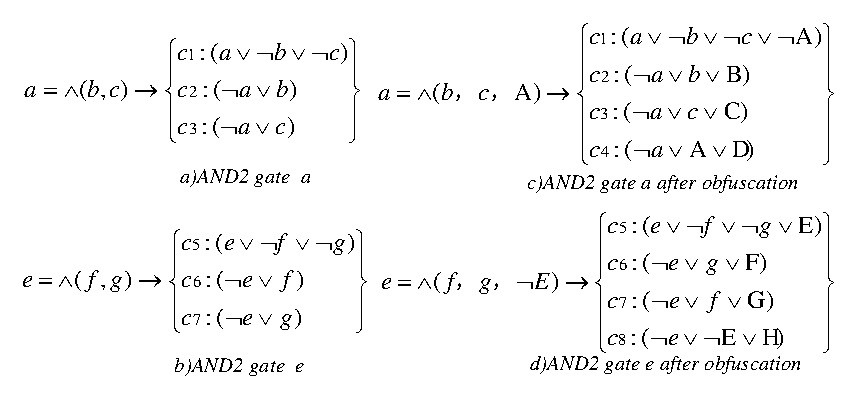
\includegraphics[width=8.2cm]{AND2-2}
\caption{混淆前后$a$和$e$的CNF标记}
%\caption{CNF signature of $a$ and $e$ before and after obfuscation}
\label{3:fig_beforeafter}
\end{figure}

图\ref{3:fig_beforeafter}a) 和\ref{3:fig_beforeafter}b) 给出了两个AND2门$a$和$e$的CNF 标记,
混淆后的标记显示在图\ref{3:fig_beforeafter}c)和\ref{3:fig_beforeafter}d) 中。
其中包括三种改变:
\begin{enumerate}
 \item
 关键子句$c_1$和$c_5$ 的长度由3变为4。
这就阻止了基于关键子句模式匹配的电路结构探测算法\upcite{csFu}的攻击;
 \item
$a$的特征子句$c_1$-$c_3$) 以及$e$的特征子句$c_5$-$c_7$变成了完全不同的形式,
并且有新的子句加入了公式,如$c_4$和$c_8$。
这就阻止了基于标记子图同构的电路结构检测算法\upcite{csRoy}的攻击;
\item
 通过加入合适的新文字以及构造新的子句,
 门$a$ 的CNF标记从AND2变为了AND3,
如图\ref{3:fig_beforeafter}a) 和\ref{3:fig_beforeafter}c)。
Husk文字$A$,
变成了新生成的AND3门的一个输入,
并且与原始AND2门的输入$b$ 和$c$不可区分。
这也使得区分混淆后AND2和真实AND3变得不再可能。
\end{enumerate}

\subsubsection{算法复杂性分析}
根据本章提出的基于混淆的SAT 求解框架,SAT问题求解开销包含私有云上的计算开销和公共云中的计算开销。
在私有云中,计算开销包括CNF 公式混淆开销和结果恢复开销;
在公共云中的计算开销是指对混淆后CNF公式的SAT 求解开销。
由于Husk公式可以预先产生,因此在本文中,Husk公式的产生开销将不再被列入到每一次SAT求解的开销中。

\textbf{混淆算法的复杂性}

%Obfuscation is implemented in Algorithm \ref{3:algo_obs}.
%The main procedure of Algorithm \ref{3:algo_obs} consists only one layer of loop,
%but one of it sub-procedure $\mathbf{mark}$ (Algorithm \ref{3:algo_mark}) consists 4 layers of loop,
%and the runtimes of the 2 inner loops are bounded by length of clauses.
%So the complexity of the obfuscation algorithm is $O(n^2)$.
算法\ref{3:algo_obs}实现了混淆,其中主程序仅仅包含一层循环,
但是其中一个子程序$\mathbf{mark}$(算法\ref{3:algo_mark})包含了4层循环,
由于两层内循环的上界为子句长度,
因此混淆算法复杂性为$O(n^2)$。

\textbf{解恢复算法的复杂性}

%Solution recovery is implemented in  Algorithm \ref{3:algo_map},
%which only consists one layer of loop,
%its complexity is $O(n)$.
%According to Theorem \ref{3:SSOtheorem}, result from SAT solver may consist false solution,
%so Algorithm \ref{3:algo_map} may be run more than one time to get correct solution.
%Since Algorithm \ref{3:algo_map} is of linear complexity,
%it incurs minor impact on performance of SAT Solving.
解恢复在算法\ref{3:algo_map}中实现,
由于仅仅包含一层循环,算法复杂度为$O(n)$。
%根据定理\ref{3:SSOtheorem}, 来自于SAT求解器的解可能包含假解,
%因此为获得正确解,算法\ref{3:algo_map}可能会运行不只一次.
由于算法\ref{3:algo_map}为线性复杂度,
带给整个求解过程的开销较小。

\subsection{实验评估}
\subsubsection{实验设计}
本文给出的算法由C语言实现。
实验用机器的配置为Intel Core(TM) i7-3667U CPU @ 2.00GHz, 8GB RAM。

将ISCAS89测试集中的部分电路,按照形式化验证时的要求分别展开20、30、100次并编码为CNF公式。
产生的Husks公式包含的节点数和子句数分别为$vn=675$和$cn=2309$。
使用MiniSat\upcite{EXTSAT}作为求解器,
模拟开放环境下隐私保护SAT求解计算。

\subsubsection{实验结果分析}
表\ref{3:fig_exp}给出了实验结果,表中各个参数的意义如下所示:
\begin{enumerate}
\item \textbf{变量数/子句数(vn/cn)}:原始CNF 公式中包含的变量数和子句数。
\item \textbf{求解时间(Solving Time)}:混淆前后的SAT问题得到第一个可满足解的时间。
\item \textbf{混淆时间(Obfuscation Time)}:按照混淆算法在原公式中混合入HUSK公式的时间。
\item \textbf{解恢复时间(Map Time)}:从混淆后的解中恢复出实际解的时间。
\end{enumerate}

实验证实了算法的正确性,对取自ISCAS89中的13个示例电路生成的可满足CNF公式,混淆前后的SAT 求解的结果一致。

依据下式定义的非对称加速比( Asymmetric~Speedup)\upcite{c.WANG},
对全部的电路,其非对称加速比均超过了100\%。
特别是某些尺寸较大的路,非对称加速比超过500%
这表明了外包复杂SAT求解函数的必要性。
\begin{equation}
%异构加速比= \frac{求解时间}{混淆时间 + 解恢复时间}
Asymmetric~Speedup= \frac{Solving~Time}{Obfuscation~Times + Map~Time}
\end{equation}

实验也显示出混淆后带来的SAT 求解的开销,不同的电路具有不同的表现。
\begin{equation}
%求解开销=\frac{混淆后求解时间-混淆前求解时间}{混淆前求解时间}
Solving~OverHead=\frac{Solving~Time~After~Obfuscation-Solving~Time~Before~Obfuscation}{Solving~Time~Before~Obfuscation}
\end{equation}
90\% 以上的电路,开销小于100\%。
仅有少部分电路,开销超过了100\%;
 这表明简单的混淆策略引入的求解开销是可以接受的。
%这些事实提醒我们两件事情:
%首先,混淆时间取决于被改变的门数,
%需要研究更加精巧的混淆算法以改变较少的门的情况下仍然可以迷惑攻击者.
%第二, 由于混淆引入的SAT求解开销,因电路而异,在设计混淆算法时,需要考虑修改后结构对求解时间的影响。

\begin{table*}
\caption{不同类型电路CNF公式混淆前后的运行时间}
%\caption{Runtime of CNF formula generated from different Circuit}
\centering
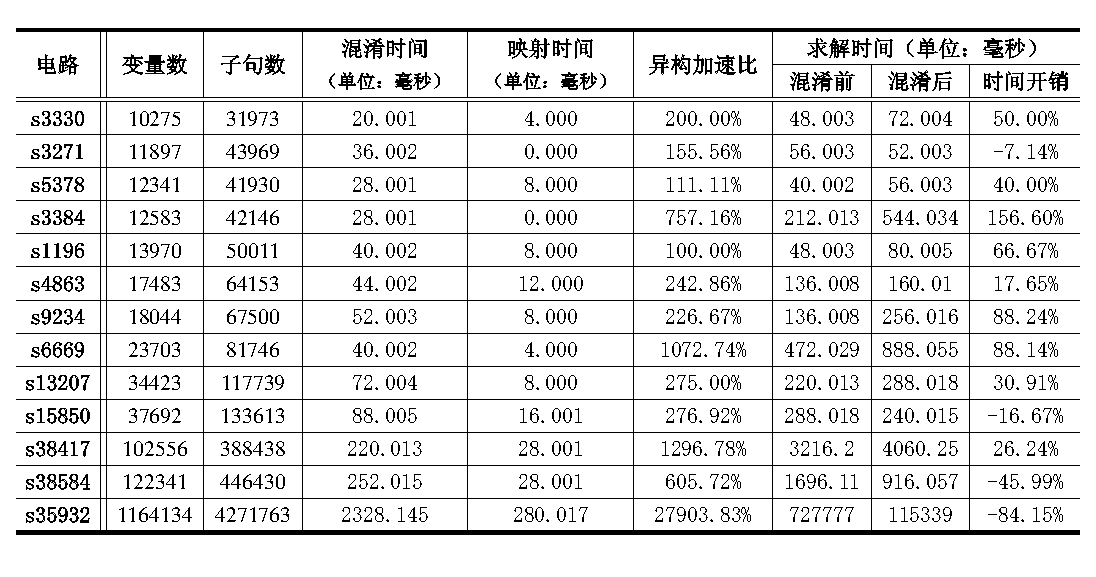
\includegraphics[width=14.2cm]{fig302}
\label{3:fig_exp}
\end{table*}%
%
%\section{Conclusion}
%This paper proposes a circuit aware  CNF obfuscation algorithm,
%that can prevent the confidential information from being recovered by adversary,
%when outsourcing SAT problem in Cloud or grid.
%Theoretical analysis and experimental results show that algorithms can significantly change structure of CNF formula,
%with polynomial complexity and without narrowing down its solution space.
\section{本章小结}
在本章中,我们对SAT求解的安全外包进行了建模,
给出了实现SAT问题求解输入隐私保护的有效方案,
并设计了结构感知的CNF混淆方法,
以防止敏感的输入信息如电路结构被恢复。
理论和实验结果都证明了方案的实用型和有效性。
%本文给出了电路结构感知的CNF混淆算法,可防止在SAT问题外包计算时,CNF公式中的电路结构以及解被窃取。
%理论分析和实验表明,算法可以有效的改变结构,同时还不会缩减CNF公式的解空间。
